\section{Threat Model}
\label{sec:thretmodel}
\begin{figure}
    \centering
    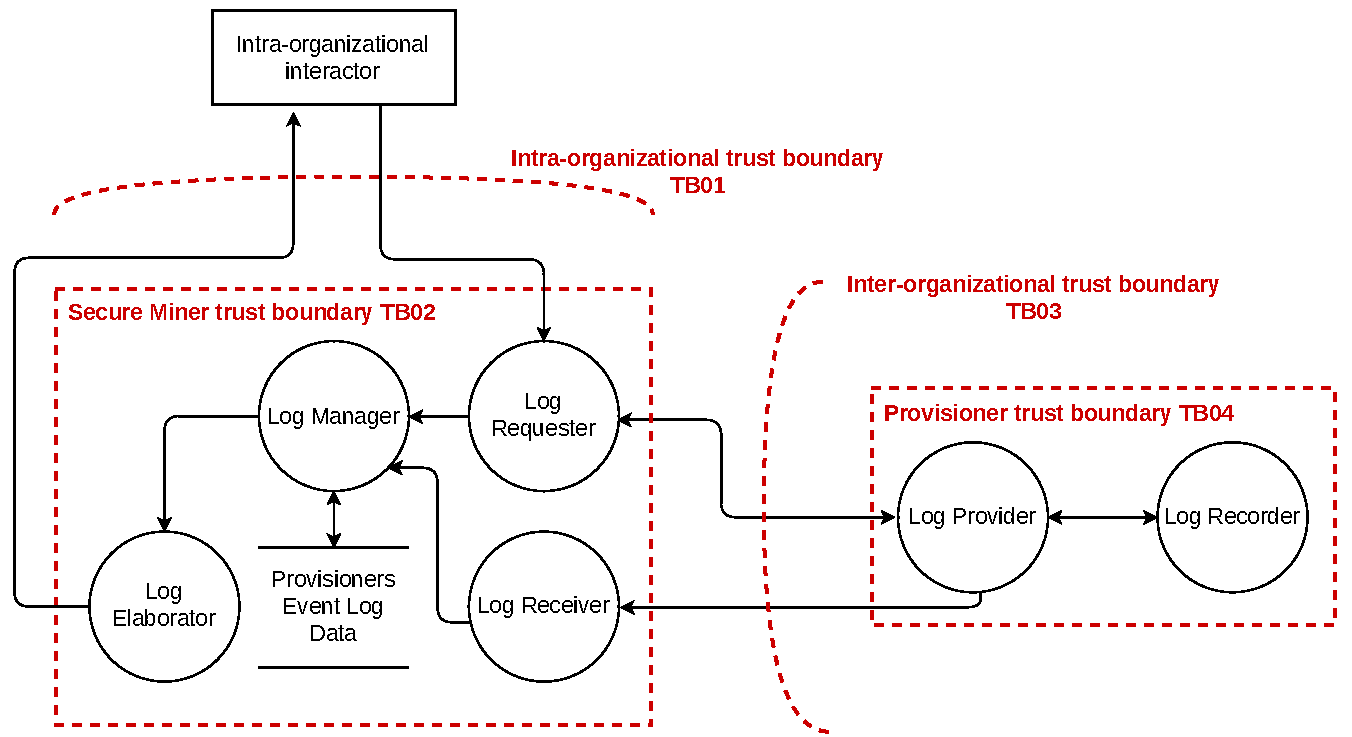
\includegraphics[width=0.95\linewidth]{content//figures/threatmodel.pdf}
    \caption{Data flow diagram employed for our threat model}
    \label{fig:threatmodel:dataflow}
\end{figure}
\begin{table}[t]
\resizebox{\textwidth}{!}{%
    \centering
    \begin{tabular}{llll}\toprule
        \textbf{ID} & \textbf{Trust boundary}& \textbf{Type}  & \textbf{Threat description}\\ \midrule
        T01& \multirow{4}{*}{\makecell[l]{TB01}}& Information disclosure  & The attacker accesses the \Compo{Secure Miner}'s memory location to leak the event logs\\ %01
        T02& & Tampering  & The attacker meddles the source code of the \Compo{Secure Miner} or its event log data\\ %02
        T03& & Elevation of privileges  & The attacker gains the rights to run in the same environment of the \Compo{Secure Miner}\\ %03
        T04& & Denial of service  & The \Compo{Secure Miner} crashes, halts or stops\\ \midrule %04
        T05& \multirow{5}{*}{\makecell[l]{TB02}}& Spoofing  & The attacker impersonates a \Compo{Secure Miner} to gain access to the \Compo{Provisioner}'s log\\ %05
        T06& & Spoofing  & The attacker impersonates a \Compo{Provisioner} to communicate with the \Compo{Secure Miner}\\ %06
        T07& & Denial of service &The \Compo{Secure Miner} floods the \Compo{Provisioner} with log requests\\ %07
        T08& & Information disclosure & The attacker sniffs the \Compo{Provisioner}'s log sent to the \Compo{Secure Miner}\\ %08
        T09& & Tampering & The attacker alters the data flow between the \Compo{Provisioner} and the \Compo{Secure Miner}\\ \midrule %09
        T10& \multirow{3}{*}{\makecell[l]{TB03}}& Spoofing   & The attacker impersonates a legitimate interactor to use the \Compo{Secure Miner}\\ %10
        T11&     & Tampering  & The intra-organizational interactor sends malicious input to the \Compo{Secure Miner}\\ %11
        T12&     & Information disclosure  & The attacker sniffs the messages between the interactor and the \Compo{Secure Miner}\\ %12
        \bottomrule
    \end{tabular}
    \caption{Vulnerabilities in the CONFINE architecture}
    \label{table:threatmodel:threats}
}
\end{table}
\begin{newj}
In the following section, we identify the threats that can jeopardize the proper functioning of the CONFINE architecture. Our threat analysis is based upon the theoretical foundation of the \textit{STRIDE} framework \cite{DBLP:journals/re/ScandariatoWJ15}. This conceptual model groups the threats into six categories: \textit{spoofing} (i.e., the impersonation of a legitimate entity), tampering (i.e., the modification of data to alter its integrity), \textit{repudiation} (i.e., the denial of performing a particular action), \textit{information disclosure} (i.e., the exposure of sensitive data), \textit{denial of service} (i.e., the disruption or degradation of availability) and \textit{elevation of privileges} (i.e., the misappropriation of higher level of rights). 

With the help of the dataflow diagram (DFD) depicted in \cref{fig:threatmodel:dataflow}, we demarcate the \textit{trust boundaries} among the CONFINE components. In our DFD, a trust boundary box (a red dashed square) groups entities with mutual trust. Differently, trust boundary arches (red dashed curved lines) mark the transitions of trust level on the occasion of data exchanges between mutually untrusted interactors. We identify four trust boundaries: the \Compo{Secure Miner}'s trust zone (\textbf{TB01}), the inter-organizational trust boundary (\textbf{TB02}), the intra-organizational trust boundary (\textbf{TB03}) and the \Compo{Provisioner}'s trust zone (\textbf{TB04}). As a result of our analysis, we collect in \cref{table:threatmodel:threats} the threats in CONFINE according to the STRIDE taxonomy.

We address the identified threats, grouping them according to the threat boundary they refer to. In our examination, we exclude the security considerations pertaining to TB04 (depicted in our DFD as a red matte box) that fall beyond the scope of this study. Therefore, we concentrate our research endeavors on the settings wherein \Compo{Provisioner}s' log partitions (introduced in \cref{def:partition}) crosses the organizational confines. 

The trust boundary box TB01 encloses the components of the \Compo{Secure Miner}. The spectrum of potential attacks targeting this trust domain aims to undermine the isolation layer that separates the components of the \Compo{Secure Miner}, including provisioners' log partitions, from untrusted entities. Attacks against this trust boundary may emanate from a generic entity, which could be either intra-organizational (i.e., within the same organization as the \Compo{Secure Miner}) or inter-organizational (i.e., beyond the boundaries of the \Compo{Secure Miner}'s organization). To expose confidential information, a malicious actor might gain access to the memory allocated to the \Compo{Secure Miner}, for instance, through a \textit{direct memory access} attack \cite{DBLP:conf/cms/EckertPK13}, thereby revealing event logs' sensitive information (\textbf{T01}). Tampering threats materialize in the form of manipulating the \Compo{Secure Miner}'s source code and event log data to induce misbehaviors or introduce vulnerabilities (\textbf{T02}). Furthermore, a malicious actor could obtain the necessary privileges, such as through \textit{kernel exploits} \cite{DBLP:conf/securecomm/XiaoHW15a}, to execute code within the isolated context of the \Compo{Secure Miner}, potentially resulting in unauthorized access or the injection of malicious code (\textbf{T03}). A denial of service attack may be employed by a malicious entity to crash, halt, or disrupt the functioning of the \Compo{Secure Miner}, thereby hindering the aggregation event log data correctly and the outsourcing of result analytics (\textbf{T04}). 

TB02  encompasses inter-organizational concerns between the \Compo{Secure Miner} and the \Compo{Provisioner}. Considering this specific setting, an attacker may disrupt the data transmission process responsible for delivering log partitions from the \Compo{Provisioner} to the \Compo{Secure Miner}. A spoofing attack could result in the \Compo{Secure Miner} being impersonated, leading to the improper reception of the \Compo{Provisioner}'s log partition (\textbf{T05}). Similarly, if an attacker successfully impersonates a \Compo{Provisioner}, it could send fictitious event logs to manipulate the data analytics output (\textbf{T06}). Furthermore, the log delivery service may be interrupted by one or more malicious entities generating an excessive number of data requests (e.g., through \textit{DDoS} \cite{DBLP:journals/ijdsn/MahjabinXSJ17} and \textit{TCP-SYN floodding} \cite{DBLP:journals/wpc/SwamiDR21} attacks) targeting the \Compo{Provisioner} (\textbf{T07}). A man-in-the-middle attack, such as eavesdropping and packet sniffing \cite{DBLP:journals/jocs/LiXDZCW15}, could allow a third-party actor to monitor the data flow between the \Compo{Secure Miner} and the \Compo{Provisioner}, thereby enabling the disclosure of event logs' confidential information (\textbf{T08}) or the alteration of meaningful data (\textbf{T09}).

Lastly, the TB03 trust boundary involves the interaction between the \Compo{Secure Miner} and a generic intra-organizational interactor within the same organization. A spoofing threat holds the potential for an assailant to emulate a legitimate interactor, enabling them to engage with the \Compo{Secure Miner} (\textbf{T10}). Furthermore, there exists a risk wherein a legitimate interactor, motivated by malicious intent, may introduce deleterious inputs to the \Compo{Secure Miner}, including the submission of corrupted data or issuance of dangerous commands (\textbf{T11}). The emergence of information disclosure threats transpires when a malicious actor intercepts messages exchanged between a legitimate interactor and the \Compo{Secure Miner}, thereby attaining unauthorized access to sensitive information, including credentials or reserved outputs (\textbf{T12}).

\end{newj}


